% Options for packages loaded elsewhere
\PassOptionsToPackage{unicode}{hyperref}
\PassOptionsToPackage{hyphens}{url}
%
\documentclass[
  ignorenonframetext,
]{beamer}
\usepackage{pgfpages}
\setbeamertemplate{caption}[numbered]
\setbeamertemplate{caption label separator}{: }
\setbeamercolor{caption name}{fg=normal text.fg}
\beamertemplatenavigationsymbolsempty
% Prevent slide breaks in the middle of a paragraph
\widowpenalties 1 10000
\raggedbottom
\setbeamertemplate{part page}{
  \centering
  \begin{beamercolorbox}[sep=16pt,center]{part title}
    \usebeamerfont{part title}\insertpart\par
  \end{beamercolorbox}
}
\setbeamertemplate{section page}{
  \centering
  \begin{beamercolorbox}[sep=12pt,center]{part title}
    \usebeamerfont{section title}\insertsection\par
  \end{beamercolorbox}
}
\setbeamertemplate{subsection page}{
  \centering
  \begin{beamercolorbox}[sep=8pt,center]{part title}
    \usebeamerfont{subsection title}\insertsubsection\par
  \end{beamercolorbox}
}
\AtBeginPart{
  \frame{\partpage}
}
\AtBeginSection{
  \ifbibliography
  \else
    \frame{\sectionpage}
  \fi
}
\AtBeginSubsection{
  \frame{\subsectionpage}
}
\usepackage{amsmath,amssymb}
\usepackage{iftex}
\ifPDFTeX
  \usepackage[T1]{fontenc}
  \usepackage[utf8]{inputenc}
  \usepackage{textcomp} % provide euro and other symbols
\else % if luatex or xetex
  \usepackage{unicode-math} % this also loads fontspec
  \defaultfontfeatures{Scale=MatchLowercase}
  \defaultfontfeatures[\rmfamily]{Ligatures=TeX,Scale=1}
\fi
\usepackage{lmodern}
\usetheme[]{CambridgeUS}
\usecolortheme{seagull}
\usefonttheme{professionalfonts}
\ifPDFTeX\else
  % xetex/luatex font selection
\fi
% Use upquote if available, for straight quotes in verbatim environments
\IfFileExists{upquote.sty}{\usepackage{upquote}}{}
\IfFileExists{microtype.sty}{% use microtype if available
  \usepackage[]{microtype}
  \UseMicrotypeSet[protrusion]{basicmath} % disable protrusion for tt fonts
}{}
\makeatletter
\@ifundefined{KOMAClassName}{% if non-KOMA class
  \IfFileExists{parskip.sty}{%
    \usepackage{parskip}
  }{% else
    \setlength{\parindent}{0pt}
    \setlength{\parskip}{6pt plus 2pt minus 1pt}}
}{% if KOMA class
  \KOMAoptions{parskip=half}}
\makeatother
\usepackage{xcolor}
\newif\ifbibliography
\usepackage{color}
\usepackage{fancyvrb}
\newcommand{\VerbBar}{|}
\newcommand{\VERB}{\Verb[commandchars=\\\{\}]}
\DefineVerbatimEnvironment{Highlighting}{Verbatim}{commandchars=\\\{\}}
% Add ',fontsize=\small' for more characters per line
\usepackage{framed}
\definecolor{shadecolor}{RGB}{248,248,248}
\newenvironment{Shaded}{\begin{snugshade}}{\end{snugshade}}
\newcommand{\AlertTok}[1]{\textcolor[rgb]{0.94,0.16,0.16}{#1}}
\newcommand{\AnnotationTok}[1]{\textcolor[rgb]{0.56,0.35,0.01}{\textbf{\textit{#1}}}}
\newcommand{\AttributeTok}[1]{\textcolor[rgb]{0.13,0.29,0.53}{#1}}
\newcommand{\BaseNTok}[1]{\textcolor[rgb]{0.00,0.00,0.81}{#1}}
\newcommand{\BuiltInTok}[1]{#1}
\newcommand{\CharTok}[1]{\textcolor[rgb]{0.31,0.60,0.02}{#1}}
\newcommand{\CommentTok}[1]{\textcolor[rgb]{0.56,0.35,0.01}{\textit{#1}}}
\newcommand{\CommentVarTok}[1]{\textcolor[rgb]{0.56,0.35,0.01}{\textbf{\textit{#1}}}}
\newcommand{\ConstantTok}[1]{\textcolor[rgb]{0.56,0.35,0.01}{#1}}
\newcommand{\ControlFlowTok}[1]{\textcolor[rgb]{0.13,0.29,0.53}{\textbf{#1}}}
\newcommand{\DataTypeTok}[1]{\textcolor[rgb]{0.13,0.29,0.53}{#1}}
\newcommand{\DecValTok}[1]{\textcolor[rgb]{0.00,0.00,0.81}{#1}}
\newcommand{\DocumentationTok}[1]{\textcolor[rgb]{0.56,0.35,0.01}{\textbf{\textit{#1}}}}
\newcommand{\ErrorTok}[1]{\textcolor[rgb]{0.64,0.00,0.00}{\textbf{#1}}}
\newcommand{\ExtensionTok}[1]{#1}
\newcommand{\FloatTok}[1]{\textcolor[rgb]{0.00,0.00,0.81}{#1}}
\newcommand{\FunctionTok}[1]{\textcolor[rgb]{0.13,0.29,0.53}{\textbf{#1}}}
\newcommand{\ImportTok}[1]{#1}
\newcommand{\InformationTok}[1]{\textcolor[rgb]{0.56,0.35,0.01}{\textbf{\textit{#1}}}}
\newcommand{\KeywordTok}[1]{\textcolor[rgb]{0.13,0.29,0.53}{\textbf{#1}}}
\newcommand{\NormalTok}[1]{#1}
\newcommand{\OperatorTok}[1]{\textcolor[rgb]{0.81,0.36,0.00}{\textbf{#1}}}
\newcommand{\OtherTok}[1]{\textcolor[rgb]{0.56,0.35,0.01}{#1}}
\newcommand{\PreprocessorTok}[1]{\textcolor[rgb]{0.56,0.35,0.01}{\textit{#1}}}
\newcommand{\RegionMarkerTok}[1]{#1}
\newcommand{\SpecialCharTok}[1]{\textcolor[rgb]{0.81,0.36,0.00}{\textbf{#1}}}
\newcommand{\SpecialStringTok}[1]{\textcolor[rgb]{0.31,0.60,0.02}{#1}}
\newcommand{\StringTok}[1]{\textcolor[rgb]{0.31,0.60,0.02}{#1}}
\newcommand{\VariableTok}[1]{\textcolor[rgb]{0.00,0.00,0.00}{#1}}
\newcommand{\VerbatimStringTok}[1]{\textcolor[rgb]{0.31,0.60,0.02}{#1}}
\newcommand{\WarningTok}[1]{\textcolor[rgb]{0.56,0.35,0.01}{\textbf{\textit{#1}}}}
\setlength{\emergencystretch}{3em} % prevent overfull lines
\providecommand{\tightlist}{%
  \setlength{\itemsep}{0pt}\setlength{\parskip}{0pt}}
\setcounter{secnumdepth}{-\maxdimen} % remove section numbering
\usepackage{placeins}
\usepackage{color}
\usepackage{bm}
\usepackage{amsmath}
\usepackage{algorithm}
\usepackage[]{algpseudocode}
\usepackage{tabularx}
\usepackage{multirow}
\usepackage[most]{tcolorbox}
\usepackage{tikz}
\usepackage{lipsum}
\usepackage{mathtools}
\usepackage{actuarialangle}
\usepackage{multirow, longtable, array, dcolumn}
\usepackage{tabu}
\newcommand{\sdt}{\bullet}
\newcommand{\tss}{\textsuperscript}
\newcommand{\morearraysp}{\setlength{\arraycolsep}{2mm}}
\newcommand{\smarraysp}{\setlength{\arraycolsep}{1mm}}
\newcommand{\oldarraysp}{\setlength{\arraycolsep}{1.5pt}}
\newcommand{\matrixstretch}{\setlength{\extrarowheight}{4pt}}
\newcommand{\matrixnostretch}{\setlength{\extrarowheight}{0pt}}
\newcommand{\gil}[1]{\textrm{\gilfont{#1}}\normalfont }
\newfont{\gilfont}{msbm10 scaled 1000}
\newcommand{\DOT}{\usebox{\biggercirc}}
\newcommand{\pv}{\wp\text{-value}}
\ifLuaTeX
  \usepackage{selnolig}  % disable illegal ligatures
\fi
\IfFileExists{bookmark.sty}{\usepackage{bookmark}}{\usepackage{hyperref}}
\IfFileExists{xurl.sty}{\usepackage{xurl}}{} % add URL line breaks if available
\urlstyle{same}
\hypersetup{
  pdftitle={STT 3850 : Chi-Square Tests},
  pdfauthor={Fall 2023},
  hidelinks,
  pdfcreator={LaTeX via pandoc}}

\title{STT 3850 : Chi-Square Tests}
\author{Fall 2023}
\date{}
\institute{Appalachian State University}

\begin{document}
\frame{\titlepage}

\hypertarget{chi-square-goodness-of-fit-tests}{%
\section{Chi-Square Goodness-of-Fit
Tests}\label{chi-square-goodness-of-fit-tests}}

\begin{frame}{Background}
\protect\hypertarget{background}{}
\begin{itemize}
\item
  Many statistical procedures require knowledge of the population from
  which the sample is taken. For example, using Student's
  \(t\)-distribution for testing a hypothesis or constructing a
  confidence interval for \(\mu\) assumes that the parent population is
  normal.
\item
  \textbf{Goodness-of-fit} (GOF) procedures are presented that will help
  to identify the distribution of the population from which the sample
  is drawn.
\item
  The null hypothesis in a goodness-of-fit test is a statement about the
  form of the cumulative distribution. When all the parameters in the
  null hypothesis are specified, the hypothesis is called
  \textbf{simple}.
\item
  Recall that in the event the null hypothesis does not completely
  specify all of the parameters of the distribution, the hypothesis is
  said to be \textbf{composite}.
\end{itemize}
\end{frame}

\begin{frame}{Background}
\protect\hypertarget{background-1}{}
\begin{itemize}
\item
  Goodness-of-fit tests are typically used when the form of the
  population is in question. In contrast to most of the statistical
  procedures discussed so far, where the goal has been to
  \textbf{reject} the null hypothesis, in a GOF test one hopes to
  \textbf{retain} the null hypothesis.
\item
  Given a single random sample of size \(n\) from an unknown population
  \(F_X\), one may wish to test the hypothesis that \(F_X\) has some
  known distribution \(F_0(x)\) for all \(x\).
\end{itemize}
\end{frame}

\begin{frame}[fragile]{Background}
\protect\hypertarget{background-2}{}
\begin{itemize}
\item
  For example, using the data frame \texttt{SOCCER} from the
  \texttt{PASWR2} package, is it reasonable to assume the number of
  goals scored during regulation time for the 232 soccer matches has a
  Poisson distribution with \(\lambda=2.5\)?
\item
  Before applying the chi-square goodness-of-fit test, the data must be
  grouped according to some scheme to form \(k\) mutually exclusive
  categories. When the null hypothesis completely specifies the
  population, the probability that a random observation will fall into
  each of the chosen or fixed categories can be computed.
\end{itemize}
\end{frame}

\begin{frame}{Background}
\protect\hypertarget{background-3}{}
\begin{itemize}
\item
  Once the probabilities for a data point to fall into each of the
  chosen or fixed categories is computed, multiplying the probabilities
  by \(n\) produces the expected counts for each category under the null
  distribution.
\item
  If the null hypothesis is true, the differences between the counts
  observed in the \(k\) categories and the counts expected in the \(k\)
  categories should be small.
\end{itemize}
\end{frame}

\begin{frame}{Background}
\protect\hypertarget{background-4}{}
\begin{itemize}
\tightlist
\item
  The test criterion for testing
  \(H_0: F_X(x) = F_0(x) \text{ for all } x\) against the alternative
  \(H_1: F_X(x) \ne F_0(x) \text{ for some } x\) when the null
  hypothesis is completely specified is
\end{itemize}

\begin{equation}
\chi_{\text{obs}}^2=\sum_{i=1}^{k} \frac{(O_k - E_k)^2}{E_k},
\end{equation}

where \(\chi_\text{obs}^2\) is the sum of the squared deviations between
what is observed \((O_k)\) and what is expected \((E_k)\) in each of the
\(k\) categories divided by what is expected in each of the \(k\)
categories. Large values of \(\chi_\text{obs}^2\) occur when the
observed data are inconsistent with the null hypothesis and thus lead to
rejection of the null hypothesis. The exact distribution of
\(\chi_\text{obs}^2\) is very complicated; however, for large \(n\),
provided all expected categories are at least 5, \(\chi_\text{obs}^2\)
is distributed approximately \(\chi^2\) with \(k-1\) degrees of freedom.
\end{frame}

\begin{frame}{Background}
\protect\hypertarget{background-5}{}
\begin{itemize}
\tightlist
\item
  NOTE: When the null hypothesis is composite, that is, not all of the
  parameters are specified, the degrees of freedom for the random
  variable \(\chi_\text{obs}^2\) are reduced by one for each parameter
  that must be estimated.
\end{itemize}
\end{frame}

\begin{frame}[fragile]{Soccer Example}
\protect\hypertarget{soccer-example}{}
Test the hypothesis that the number of goals scored during regulation
time for the 232 soccer matches stored in the data frame \texttt{SOCCER}
has a Poisson \texttt{cdf} with \(\lambda=2.5\) with the chi-square
goodness-of-fit test and an \(\alpha\) level of 0.05. Produce a
histogram showing the number of observed goals scored during regulation
time and superimpose on the histogram the number of goals that are
expected to be made when the distribution of goals follows a Poisson
distribution with \(\lambda=2.5\).
\end{frame}

\begin{frame}[fragile]{Soccer Solution}
\protect\hypertarget{soccer-solution}{}
\begin{itemize}
\tightlist
\item
  Since the number of categories for a Poisson distribution is
  theoretically infinite, a table is first constructed of the observed
  number of goals to get an idea of reasonable categories.
\end{itemize}

\begin{Shaded}
\begin{Highlighting}[]
\FunctionTok{library}\NormalTok{(PASWR2)}
\FunctionTok{xtabs}\NormalTok{(}\SpecialCharTok{\textasciitilde{}}\NormalTok{goals, }\AttributeTok{data =}\NormalTok{ SOCCER)}
\end{Highlighting}
\end{Shaded}

\begin{verbatim}
goals
 0  1  2  3  4  5  6  7  8 
19 49 60 47 32 18  3  3  1 
\end{verbatim}
\end{frame}

\begin{frame}[fragile]{Soccer Solution}
\protect\hypertarget{soccer-solution-1}{}
Based on the table, a decision is made to create categories for 0, 1, 2,
3, 4, 5, and 6 or more goals. Under the null hypothesis that \(F_0(x)\)
is a Poisson distribution with \(\lambda=2.5\), the probabilities of
scoring 0, 1, 2, 3, 4, 5, and 6 or more goals are computed with
\texttt{R} as follows:

\begin{Shaded}
\begin{Highlighting}[]
\NormalTok{PX }\OtherTok{\textless{}{-}} \FunctionTok{c}\NormalTok{(}\FunctionTok{dpois}\NormalTok{(}\DecValTok{0}\SpecialCharTok{:}\DecValTok{5}\NormalTok{, }\FloatTok{2.5}\NormalTok{), }\FunctionTok{ppois}\NormalTok{(}\DecValTok{5}\NormalTok{, }\FloatTok{2.5}\NormalTok{, }\AttributeTok{lower =} \ConstantTok{FALSE}\NormalTok{))}
\NormalTok{PX[}\DecValTok{1}\SpecialCharTok{:}\DecValTok{4}\NormalTok{] }\CommentTok{\# Probabilities for categories 0, 1, 2, 3}
\end{Highlighting}
\end{Shaded}

\begin{verbatim}
[1] 0.0820850 0.2052125 0.2565156 0.2137630
\end{verbatim}

\begin{Shaded}
\begin{Highlighting}[]
\NormalTok{PX[}\DecValTok{4}\SpecialCharTok{:}\DecValTok{6}\NormalTok{] }\CommentTok{\# Probabilities for categories 4, 5, and 6 or more}
\end{Highlighting}
\end{Shaded}

\begin{verbatim}
[1] 0.21376302 0.13360189 0.06680094
\end{verbatim}
\end{frame}

\begin{frame}[fragile]{Soccer Solution}
\protect\hypertarget{soccer-solution-2}{}
\begin{tcolorbox}
Since there were a total of $n=232$ soccer games, the expected
number of goals for the six categories is simply $232 \times
\tt{PX}$.
\end{tcolorbox}

\begin{Shaded}
\begin{Highlighting}[]
\NormalTok{EX }\OtherTok{\textless{}{-}} \DecValTok{232}\SpecialCharTok{*}\NormalTok{PX}
\NormalTok{OB }\OtherTok{\textless{}{-}} \FunctionTok{c}\NormalTok{(}\FunctionTok{as.vector}\NormalTok{(}\FunctionTok{xtabs}\NormalTok{(}\SpecialCharTok{\textasciitilde{}}\NormalTok{goals, }\AttributeTok{data =}\NormalTok{ SOCCER)[}\DecValTok{1}\SpecialCharTok{:}\DecValTok{6}\NormalTok{]), }
        \FunctionTok{sum}\NormalTok{(}\FunctionTok{xtabs}\NormalTok{(}\SpecialCharTok{\textasciitilde{}}\NormalTok{goals, }\AttributeTok{data =}\NormalTok{ SOCCER)[}\DecValTok{7}\SpecialCharTok{:}\DecValTok{9}\NormalTok{]))}
\NormalTok{OB}
\end{Highlighting}
\end{Shaded}

\begin{verbatim}
[1] 19 49 60 47 32 18  7
\end{verbatim}

\begin{Shaded}
\begin{Highlighting}[]
\NormalTok{ans }\OtherTok{\textless{}{-}} \FunctionTok{cbind}\NormalTok{(PX, EX, OB)}
\FunctionTok{row.names}\NormalTok{(ans) }\OtherTok{\textless{}{-}} \FunctionTok{c}\NormalTok{(}\StringTok{" X=0"}\NormalTok{,}\StringTok{" X=1"}\NormalTok{,}\StringTok{" X=2"}\NormalTok{, }
                    \StringTok{" X=3"}\NormalTok{,}\StringTok{" X=4"}\NormalTok{,}\StringTok{" X=5"}\NormalTok{,}\StringTok{"X\textgreater{}=6"}\NormalTok{)}
\end{Highlighting}
\end{Shaded}
\end{frame}

\begin{frame}[fragile]{Soccer Solution}
\protect\hypertarget{soccer-solution-3}{}
\begin{Shaded}
\begin{Highlighting}[]
\NormalTok{ans}
\end{Highlighting}
\end{Shaded}

\begin{verbatim}
             PX        EX OB
 X=0 0.08208500 19.043720 19
 X=1 0.20521250 47.609299 49
 X=2 0.25651562 59.511624 60
 X=3 0.21376302 49.593020 47
 X=4 0.13360189 30.995638 32
 X=5 0.06680094 15.497819 18
X>=6 0.04202104  9.748881  7
\end{verbatim}
\end{frame}

\begin{frame}[fragile]{Soccer Solution}
\protect\hypertarget{soccer-solution-4}{}
The null and alternative hypotheses for using the chi-square
goodness-of-fit test to test the hypothesis that the number of goals
scored during regulation time for the 232 soccer matches stored in the
data frame \texttt{SOCCER} has a Poisson \texttt{cdf} with
\(\lambda=2.5\) are

\begin{align*}
        H_0&: F_X(x) = F_0(x) \sim Pois(\lambda=2.5)\text{ for all } x \text{ versus
        }\\
        H_1&:  F_X(x) \ne F_0(x) \text{ for some } x.
\end{align*}
\end{frame}

\begin{frame}[fragile]{Soccer Solution}
\protect\hypertarget{soccer-solution-5}{}
\begin{itemize}
\item
  The test statistic chosen is \(\chi_{\text{obs}}^2.\)
\item
  Reject if \(\chi^2_{\text{obs}}>\chi^2_{1-\alpha;k-1}\).
\end{itemize}

\begin{Shaded}
\begin{Highlighting}[]
\NormalTok{chi.obs }\OtherTok{\textless{}{-}} \FunctionTok{sum}\NormalTok{((OB}\SpecialCharTok{{-}}\NormalTok{EX)}\SpecialCharTok{\^{}}\DecValTok{2}\SpecialCharTok{/}\NormalTok{EX)}
\NormalTok{chi.obs}
\end{Highlighting}
\end{Shaded}

\begin{verbatim}
[1] 1.39194
\end{verbatim}
\end{frame}

\begin{frame}[fragile]{Soccer Solution}
\protect\hypertarget{soccer-solution-6}{}
\begin{Shaded}
\begin{Highlighting}[]
\FunctionTok{chisq.test}\NormalTok{(}\AttributeTok{x =}\NormalTok{ OB, }\AttributeTok{p =}\NormalTok{ PX)}
\end{Highlighting}
\end{Shaded}

\begin{verbatim}

    Chi-squared test for given probabilities

data:  OB
X-squared = 1.3919, df = 6, p-value = 0.9663
\end{verbatim}
\end{frame}

\begin{frame}[fragile]{Soccer Solution}
\protect\hypertarget{soccer-solution-7}{}
\(1.3919402=\chi^2_{\text{obs}}\overset{?}{>}\chi^2_{0.95;6}=12.5915872\).

The \(p\)-value is 0.9663469.

\begin{Shaded}
\begin{Highlighting}[]
\NormalTok{p.val }\OtherTok{\textless{}{-}} \FunctionTok{pchisq}\NormalTok{(chi.obs, }\DecValTok{7{-}1}\NormalTok{, }\AttributeTok{lower =} \ConstantTok{FALSE}\NormalTok{)}
\NormalTok{p.val}
\end{Highlighting}
\end{Shaded}

\begin{verbatim}
[1] 0.9663469
\end{verbatim}
\end{frame}

\begin{frame}{Soccer Solution}
\protect\hypertarget{soccer-solution-8}{}
\begin{itemize}
\item
  Since \(\chi^2_{\text{obs}}= 1.3919402\) is not greater than
  \(\chi^2_{0.95;6}=12.5915872\), fail to reject \(H_0\).
\item
  Since the \(p\)-value = 0.9663469 is greater than 0.05, fail to reject
  \(H_0\).
\end{itemize}
\end{frame}

\begin{frame}{Soccer Solution}
\protect\hypertarget{soccer-solution-9}{}
\begin{tcolorbox}
\textbf{English Conclusion:} There is no evidence to suggest that the true \textbf{cdf} does not equal the Poisson 
distribution with $\lambda=2.5$ for at least one $x$.
\end{tcolorbox}
\end{frame}

\begin{frame}[fragile]{Soccer Solution}
\protect\hypertarget{soccer-solution-10}{}
The following code can be used to create a histogram with superimposed
expected goals.

\begin{Shaded}
\begin{Highlighting}[]
\FunctionTok{hist}\NormalTok{(SOCCER}\SpecialCharTok{$}\NormalTok{goals, }\AttributeTok{breaks =} \FunctionTok{c}\NormalTok{((}\SpecialCharTok{{-}}\FloatTok{0.5} \SpecialCharTok{+} \DecValTok{0}\NormalTok{)}\SpecialCharTok{:}\NormalTok{(}\DecValTok{8} \SpecialCharTok{+} \FloatTok{0.5}\NormalTok{)), }
     \AttributeTok{col =} \StringTok{"lightblue"}\NormalTok{, }
     \AttributeTok{xlab =} \StringTok{"Goals scored"}\NormalTok{, }\AttributeTok{ylab =} \StringTok{""}\NormalTok{, }
     \AttributeTok{freq =} \ConstantTok{TRUE}\NormalTok{, }\AttributeTok{main =} \StringTok{""}\NormalTok{)}
\NormalTok{x }\OtherTok{\textless{}{-}} \DecValTok{0}\SpecialCharTok{:}\DecValTok{8}
\NormalTok{fx }\OtherTok{\textless{}{-}}\NormalTok{ (}\FunctionTok{dpois}\NormalTok{(}\DecValTok{0}\SpecialCharTok{:}\DecValTok{8}\NormalTok{, }\AttributeTok{lambda =} \FloatTok{2.5}\NormalTok{))}\SpecialCharTok{*}\DecValTok{232}
\FunctionTok{lines}\NormalTok{(x, fx, }\AttributeTok{type =} \StringTok{"h"}\NormalTok{)}
\FunctionTok{lines}\NormalTok{(x, fx, }\AttributeTok{type =} \StringTok{"p"}\NormalTok{, }\AttributeTok{pch =} \DecValTok{16}\NormalTok{)}
\end{Highlighting}
\end{Shaded}
\end{frame}

\begin{frame}{Soccer Solution}
\protect\hypertarget{soccer-solution-11}{}
\begin{center}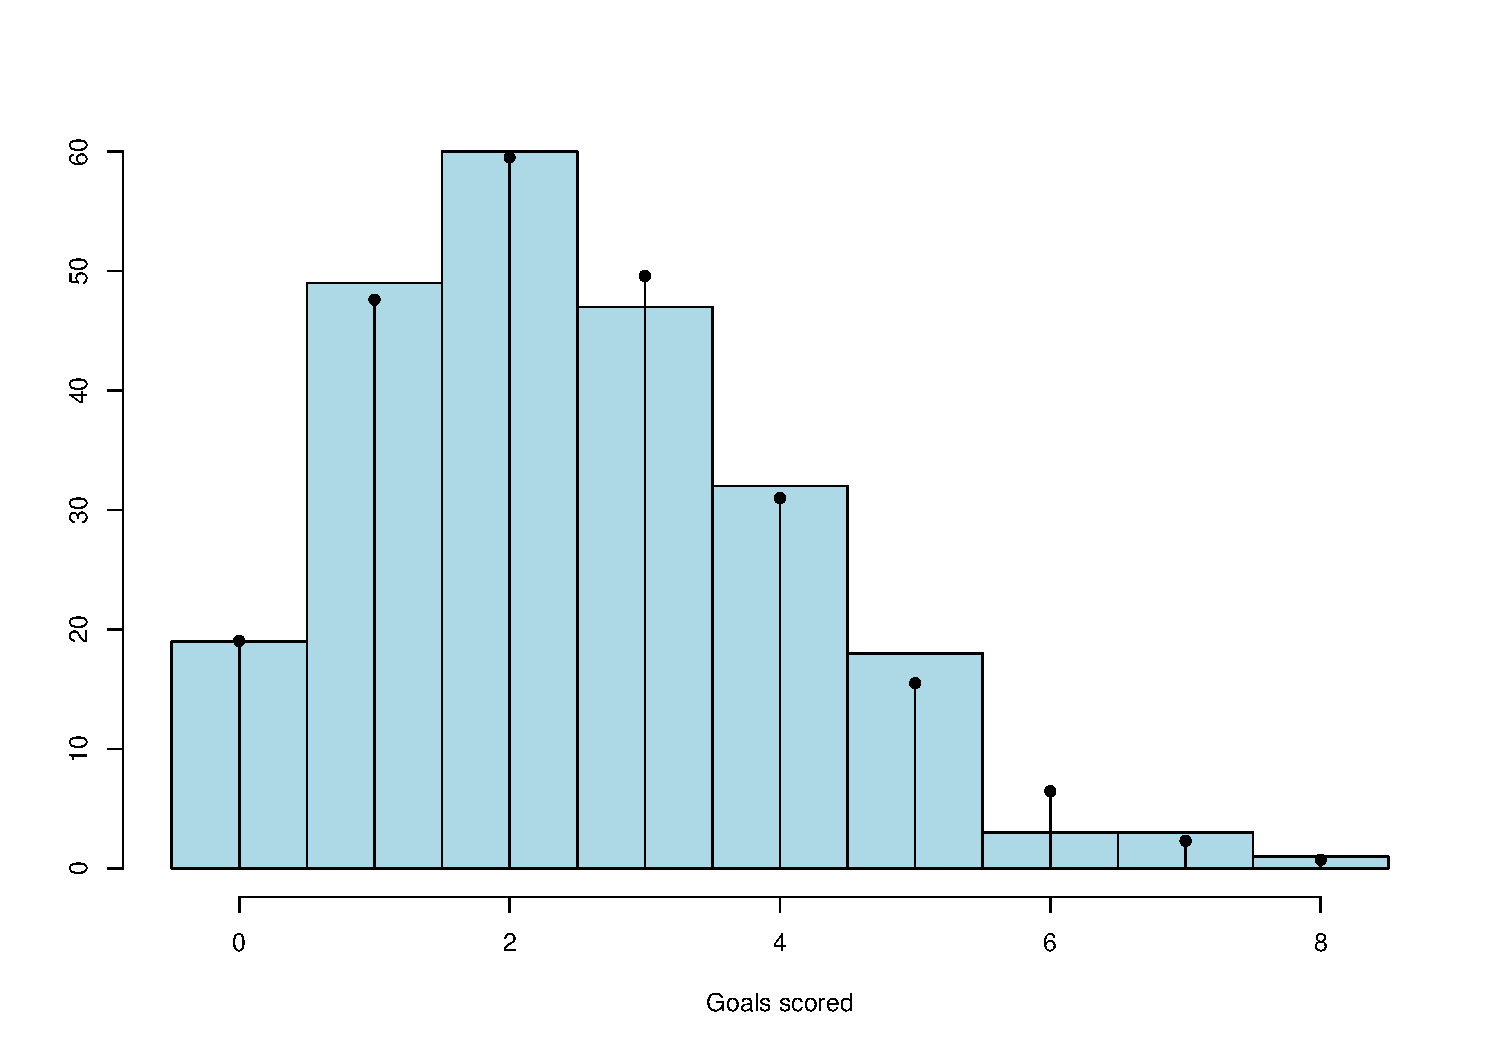
\includegraphics[width=0.85\linewidth,height=0.65\textheight]{ChiSquareTests_files/figure-beamer/unnamed-chunk-9-1} \end{center}
\end{frame}

\begin{frame}[fragile]{All Parameters Known}
\protect\hypertarget{all-parameters-known}{}
\begin{itemize}
\tightlist
\item
  Bansley et al.~(1992) investigated the relationship between month of
  birth and achievement in sport. Birth dates were collected for players
  in teams competing in the 1990 World Cup soccer games.
\end{itemize}

\begin{Shaded}
\begin{Highlighting}[]
\NormalTok{Observed }\OtherTok{\textless{}{-}} \FunctionTok{c}\NormalTok{(}\DecValTok{150}\NormalTok{, }\DecValTok{138}\NormalTok{, }\DecValTok{140}\NormalTok{, }\DecValTok{100}\NormalTok{)}
\FunctionTok{names}\NormalTok{(Observed) }\OtherTok{\textless{}{-}} \FunctionTok{c}\NormalTok{(}\StringTok{"Aug{-}Oct"}\NormalTok{, }\StringTok{"Nov{-}Jan"}\NormalTok{, }
                     \StringTok{"Feb{-}April"}\NormalTok{, }\StringTok{"May{-}July"}\NormalTok{)}
\NormalTok{Observed}
\end{Highlighting}
\end{Shaded}

\begin{verbatim}
  Aug-Oct   Nov-Jan Feb-April  May-July 
      150       138       140       100 
\end{verbatim}
\end{frame}

\begin{frame}{All Parameters Known}
\protect\hypertarget{all-parameters-known-1}{}
We wish to test whether these data are consistent with the hypothesis
that birthdays of soccer players are uniformly distributed across the
four quarters of the year. Let \(P_i\) denote the probability of a birth
occurring in the \(i^{th}\) quarter; the hypotheses are as follows:

\(H_0: p_1=\frac{1}{4}, p_2=\frac{1}{4}, p_3=\frac{1}{4}, p_4=\frac{1}{4}\)
versus \(H_A: p_i \neq \frac{1}{4}\) for at least one \(i\).

There were a total of \(n = 528\) players considered for this study, so
the expected count for each quarter is \(528/4 = 132\).
\end{frame}

\begin{frame}[fragile]{All Parameters Known}
\protect\hypertarget{all-parameters-known-2}{}
\(\chi^2_{obs} = \sum_{i=1}^k\frac{(O_i - E_i)^2}{E_i} = \frac{(150 - 132)^2}{132} + \frac{(138 - 132)^2}{132} + \frac{(140 - 132)^2}{132} + \frac{(100 - 132)^2}{132} = 10.97\)

\begin{Shaded}
\begin{Highlighting}[]
\NormalTok{(chi\_obs }\OtherTok{\textless{}{-}} \FunctionTok{sum}\NormalTok{((Observed }\SpecialCharTok{{-}} \DecValTok{132}\NormalTok{)}\SpecialCharTok{\^{}}\DecValTok{2}\SpecialCharTok{/}\DecValTok{132}\NormalTok{))}
\end{Highlighting}
\end{Shaded}

\begin{verbatim}
[1] 10.9697
\end{verbatim}

\begin{Shaded}
\begin{Highlighting}[]
\CommentTok{\# Or}
\FunctionTok{chisq.test}\NormalTok{(Observed, }\AttributeTok{p =} \FunctionTok{c}\NormalTok{(}\DecValTok{1}\SpecialCharTok{/}\DecValTok{4}\NormalTok{, }\DecValTok{1}\SpecialCharTok{/}\DecValTok{4}\NormalTok{, }\DecValTok{1}\SpecialCharTok{/}\DecValTok{4}\NormalTok{, }\DecValTok{1}\SpecialCharTok{/}\DecValTok{4}\NormalTok{))}\SpecialCharTok{$}\NormalTok{stat}
\end{Highlighting}
\end{Shaded}

\begin{verbatim}
X-squared 
  10.9697 
\end{verbatim}
\end{frame}

\begin{frame}[fragile]{All Parameters Known}
\protect\hypertarget{all-parameters-known-3}{}
\begin{Shaded}
\begin{Highlighting}[]
\FunctionTok{chisq.test}\NormalTok{(Observed, }\AttributeTok{p =} \FunctionTok{c}\NormalTok{(}\DecValTok{1}\SpecialCharTok{/}\DecValTok{4}\NormalTok{, }\DecValTok{1}\SpecialCharTok{/}\DecValTok{4}\NormalTok{, }\DecValTok{1}\SpecialCharTok{/}\DecValTok{4}\NormalTok{, }\DecValTok{1}\SpecialCharTok{/}\DecValTok{4}\NormalTok{)) }\OtherTok{{-}\textgreater{}}\NormalTok{ CST}
\NormalTok{CST}
\end{Highlighting}
\end{Shaded}

\begin{verbatim}

    Chi-squared test for given probabilities

data:  Observed
X-squared = 10.97, df = 3, p-value = 0.01189
\end{verbatim}

\begin{Shaded}
\begin{Highlighting}[]
\NormalTok{CST}\SpecialCharTok{$}\NormalTok{observed}
\end{Highlighting}
\end{Shaded}

\begin{verbatim}
  Aug-Oct   Nov-Jan Feb-April  May-July 
      150       138       140       100 
\end{verbatim}

\begin{Shaded}
\begin{Highlighting}[]
\NormalTok{CST}\SpecialCharTok{$}\NormalTok{expected}
\end{Highlighting}
\end{Shaded}

\begin{verbatim}
  Aug-Oct   Nov-Jan Feb-April  May-July 
      132       132       132       132 
\end{verbatim}
\end{frame}

\begin{frame}[fragile]{All Parameters Known}
\protect\hypertarget{all-parameters-known-4}{}
\begin{Shaded}
\begin{Highlighting}[]
\NormalTok{(pvalue }\OtherTok{\textless{}{-}} \FunctionTok{pchisq}\NormalTok{(CST}\SpecialCharTok{$}\NormalTok{stat, }\DecValTok{3}\NormalTok{, }\AttributeTok{lower =} \ConstantTok{FALSE}\NormalTok{))}
\end{Highlighting}
\end{Shaded}

\begin{verbatim}
 X-squared 
0.01189087 
\end{verbatim}

\begin{Shaded}
\begin{Highlighting}[]
\CommentTok{\# Or}
\NormalTok{CST}\SpecialCharTok{$}\NormalTok{p.value}
\end{Highlighting}
\end{Shaded}

\begin{verbatim}
[1] 0.01189087
\end{verbatim}
\end{frame}

\begin{frame}{All Parameters Known - Conclusion}
\protect\hypertarget{all-parameters-known---conclusion}{}
\begin{tcolorbox}
Given the $p-value$ of $0.012$ evidence suggests birthdays for World Cup soccer players are not uniformly distributed.
\end{tcolorbox}
\end{frame}

\begin{frame}{All Parameters Known - Example 2}
\protect\hypertarget{all-parameters-known---example-2}{}
Suppose you draw 100 numbers at random from an unknown distribution.
Thirty values fall in the interval \((0, 0.25]\), 30 fall in
\((0.25, 0.75]\), 22 fall in \((0.75, 1.25]\), and the rest fall in
\((1.25, \infty]\). Your friend claims that the distribution is
exponential with parameter \(\lambda = 1\). Do you believe her?

\begin{itemize}
\tightlist
\item
  A random variable \(X\) has the exponential distribution with
  parameter \(\lambda > 0\) if its \textbf{pdf} is
\end{itemize}

\[f(x) = \lambda e^{-\lambda x},\quad x \geq 0.\]
\end{frame}

\begin{frame}{All Parameters Known - Example 2}
\protect\hypertarget{all-parameters-known---example-2-1}{}
We wish to test the following:

\begin{tcolorbox}
$H_0:$ The data are from an exponential distribution with $\lambda = 1$.

$H_A:$ The data are not from an exponential distribution with $\lambda = 1$.
\end{tcolorbox}
\end{frame}

\begin{frame}{All Parameters Known - Example 2}
\protect\hypertarget{all-parameters-known---example-2-2}{}
Given \(X \sim \text{Exp}(\lambda = 1)\). The probabilities for each
interval are as follows:

\(p_1 = P(0 \leq X \leq 0.25)=\int_0^{0.25}e^{-x}\,dx =0.2211992\)

\(p_2 = P(0.25 \leq X \leq 0.75)=\int_{0.25}^{0.75}e^{-x}\,dx =0.3064342\)

\(p_3 = P(0.75 \leq X \leq 1.25)=\int_{0.75}^{1.25}e^{-x}\,dx =0.1858618\)

\(p_4 = P(1.25 \leq X \leq \infty)=\int_{1.25}^{\infty}e^{-x}\,dx =0.2865048\)
\end{frame}

\begin{frame}[fragile]{All Parameters Known - Example 2}
\protect\hypertarget{all-parameters-known---example-2-3}{}
\begin{Shaded}
\begin{Highlighting}[]
\NormalTok{p1 }\OtherTok{\textless{}{-}} \FunctionTok{pexp}\NormalTok{(}\FloatTok{0.25}\NormalTok{, }\DecValTok{1}\NormalTok{)}
\NormalTok{p2 }\OtherTok{\textless{}{-}} \FunctionTok{pexp}\NormalTok{(}\FloatTok{0.75}\NormalTok{, }\DecValTok{1}\NormalTok{) }\SpecialCharTok{{-}} \FunctionTok{pexp}\NormalTok{(}\FloatTok{0.25}\NormalTok{, }\DecValTok{1}\NormalTok{)}
\NormalTok{p3 }\OtherTok{\textless{}{-}} \FunctionTok{pexp}\NormalTok{(}\FloatTok{1.25}\NormalTok{, }\DecValTok{1}\NormalTok{) }\SpecialCharTok{{-}} \FunctionTok{pexp}\NormalTok{(}\FloatTok{0.75}\NormalTok{, }\DecValTok{1}\NormalTok{)}
\NormalTok{p4 }\OtherTok{\textless{}{-}} \FunctionTok{pexp}\NormalTok{(}\FloatTok{1.25}\NormalTok{, }\DecValTok{1}\NormalTok{, }\AttributeTok{lower =} \ConstantTok{FALSE}\NormalTok{)}
\NormalTok{ps }\OtherTok{\textless{}{-}} \FunctionTok{c}\NormalTok{(p1, p2, p3, p4)}
\NormalTok{ps}
\end{Highlighting}
\end{Shaded}

\begin{verbatim}
[1] 0.2211992 0.3064342 0.1858618 0.2865048
\end{verbatim}
\end{frame}

\begin{frame}[fragile]{All Parameters Known - Example 2}
\protect\hypertarget{all-parameters-known---example-2-4}{}
\begin{Shaded}
\begin{Highlighting}[]
\NormalTok{EXP }\OtherTok{\textless{}{-}}\NormalTok{ ps}\SpecialCharTok{*}\DecValTok{100}
\NormalTok{EXP}
\end{Highlighting}
\end{Shaded}

\begin{verbatim}
[1] 22.11992 30.64342 18.58618 28.65048
\end{verbatim}

\begin{Shaded}
\begin{Highlighting}[]
\NormalTok{OBS }\OtherTok{\textless{}{-}} \FunctionTok{c}\NormalTok{(}\DecValTok{30}\NormalTok{, }\DecValTok{30}\NormalTok{, }\DecValTok{22}\NormalTok{, }\DecValTok{18}\NormalTok{)}
\NormalTok{test\_stat }\OtherTok{\textless{}{-}} \FunctionTok{sum}\NormalTok{((OBS }\SpecialCharTok{{-}}\NormalTok{ EXP)}\SpecialCharTok{\^{}}\DecValTok{2}\SpecialCharTok{/}\NormalTok{EXP)}
\NormalTok{test\_stat}
\end{Highlighting}
\end{Shaded}

\begin{verbatim}
[1] 7.406963
\end{verbatim}
\end{frame}

\begin{frame}[fragile]{All Parameters Known - Example 2}
\protect\hypertarget{all-parameters-known---example-2-5}{}
\begin{Shaded}
\begin{Highlighting}[]
\CommentTok{\# Another approach}
\FunctionTok{chisq.test}\NormalTok{(OBS, }\AttributeTok{p =}\NormalTok{ ps)}
\end{Highlighting}
\end{Shaded}

\begin{verbatim}

    Chi-squared test for given probabilities

data:  OBS
X-squared = 7.407, df = 3, p-value = 0.06
\end{verbatim}

\begin{Shaded}
\begin{Highlighting}[]
\NormalTok{pvalue }\OtherTok{\textless{}{-}} \FunctionTok{chisq.test}\NormalTok{(OBS, }\AttributeTok{p =}\NormalTok{ ps)}\SpecialCharTok{$}\NormalTok{p.value}
\NormalTok{pvalue}
\end{Highlighting}
\end{Shaded}

\begin{verbatim}
[1] 0.05999777
\end{verbatim}
\end{frame}

\begin{frame}{All Parameters Known - Example 2 - Conclusion}
\protect\hypertarget{all-parameters-known---example-2---conclusion}{}
\begin{tcolorbox}
If you test using $\alpha = 0.05$, you will fail to reject the null hypothesis since the $p-value$ $= 0.0599 > \alpha = 0.05$.  There is not convincing evidence that the data do not come from an Exp($\lambda = 1$).
\end{tcolorbox}
\end{frame}

\hypertarget{categorical-data}{%
\section{Categorical Data}\label{categorical-data}}

\begin{frame}{Different Scenarios}
\protect\hypertarget{different-scenarios}{}
The \(2 \times 2\) contingency table can be generalized for \(I\) rows
and \(J\) columns and is referred to as an \(I \times J\) contingency
table. The sampling scheme employed to acquire the information in the
table will determine the type of hypothesis that can be tested. Consider
the following two scenarios:
\end{frame}

\begin{frame}{Scenario One:}
\protect\hypertarget{scenario-one}{}
SCENARIO ONE: Is there an association between gender and a person's
happiness? To investigate whether happiness depends on gender, one might
use information collected from the General Social Survey (GSS)
(\href{http://sda.berkeley.edu/GSS}{http://sda.berkeley.edu/GSS}). In
each survey, the GSS asks, ``Taken all together, how would you say
things are these days --- would you say that you are very happy, pretty
happy, or not too happy?'\,' Respondents to each survey are coded as
either male or female. The information in the next slide shows how a
subset of respondents (26-year-olds) were classified with respect to the
variables HAPPY and SEX.
\end{frame}

\begin{frame}[fragile]{Scenario One:}
\protect\hypertarget{scenario-one-1}{}
\begin{Shaded}
\begin{Highlighting}[]
\NormalTok{HA }\OtherTok{\textless{}{-}} \FunctionTok{c}\NormalTok{(}\DecValTok{110}\NormalTok{, }\DecValTok{277}\NormalTok{, }\DecValTok{50}\NormalTok{, }\DecValTok{163}\NormalTok{, }\DecValTok{302}\NormalTok{, }\DecValTok{63}\NormalTok{)}
\NormalTok{HAT }\OtherTok{\textless{}{-}} \FunctionTok{matrix}\NormalTok{(}\AttributeTok{data =}\NormalTok{ HA, }\AttributeTok{nrow =} \DecValTok{2}\NormalTok{, }\AttributeTok{byrow =} \ConstantTok{TRUE}\NormalTok{)}
\FunctionTok{dimnames}\NormalTok{(HAT) }\OtherTok{\textless{}{-}} \FunctionTok{list}\NormalTok{(}\AttributeTok{SEX =} \FunctionTok{c}\NormalTok{(}\StringTok{"Male"}\NormalTok{, }\StringTok{"Female"}\NormalTok{),}
 \AttributeTok{Category =} \FunctionTok{c}\NormalTok{(}\StringTok{"Very Happy"}\NormalTok{, }\StringTok{"Pretty Happy"}\NormalTok{, }\StringTok{"Not To Happy"}\NormalTok{))}
\NormalTok{HAT}
\end{Highlighting}
\end{Shaded}

\begin{verbatim}
        Category
SEX      Very Happy Pretty Happy Not To Happy
  Male          110          277           50
  Female        163          302           63
\end{verbatim}
\end{frame}

\begin{frame}[fragile]{Scenario One - Expected Values}
\protect\hypertarget{scenario-one---expected-values}{}
\begin{Shaded}
\begin{Highlighting}[]
\NormalTok{E }\OtherTok{\textless{}{-}} \FunctionTok{outer}\NormalTok{(}\FunctionTok{rowSums}\NormalTok{(HAT), }\FunctionTok{colSums}\NormalTok{(HAT), }\StringTok{"*"}\NormalTok{)}\SpecialCharTok{/}\FunctionTok{sum}\NormalTok{(HAT)}
\NormalTok{E}
\end{Highlighting}
\end{Shaded}

\begin{verbatim}
       Very Happy Pretty Happy Not To Happy
Male      123.628        262.2     51.17202
Female    149.372        316.8     61.82798
\end{verbatim}

\begin{Shaded}
\begin{Highlighting}[]
\CommentTok{\# OR}
\FunctionTok{chisq.test}\NormalTok{(HAT)}\SpecialCharTok{$}\NormalTok{expected}
\end{Highlighting}
\end{Shaded}

\begin{verbatim}
        Category
SEX      Very Happy Pretty Happy Not To Happy
  Male      123.628        262.2     51.17202
  Female    149.372        316.8     61.82798
\end{verbatim}
\end{frame}

\begin{frame}{Scenario Two}
\protect\hypertarget{scenario-two}{}
SCENARIO TWO: In a double blind randomized drug trial (neither the
patient nor the physician evaluating the patient knows the treatment,
drug or placebo, the patient receives), 400 male patients with mild
dementia were randomly divided into two groups of 200. One group was
given a placebo over three months while the second group received an
experimental drug for three months. At the end of the three months, the
physicians (all psychiatrists) classified the 400 patients into one of
three categories: improved, no change, or worse. The information on the
next slide shows how the pschiatrists classified the patients. Are the
proportions in the three status categories the same for the two
treatments?
\end{frame}

\begin{frame}[fragile]{Scenario Two}
\protect\hypertarget{scenario-two-1}{}
\begin{Shaded}
\begin{Highlighting}[]
\NormalTok{DT }\OtherTok{\textless{}{-}} \FunctionTok{c}\NormalTok{(}\DecValTok{67}\NormalTok{, }\DecValTok{76}\NormalTok{, }\DecValTok{57}\NormalTok{, }\DecValTok{48}\NormalTok{, }\DecValTok{73}\NormalTok{, }\DecValTok{79}\NormalTok{)}
\NormalTok{DTT }\OtherTok{\textless{}{-}} \FunctionTok{matrix}\NormalTok{(}\AttributeTok{data =}\NormalTok{ DT, }\AttributeTok{nrow =} \DecValTok{2}\NormalTok{, }\AttributeTok{byrow =} \ConstantTok{TRUE}\NormalTok{)}
\FunctionTok{dimnames}\NormalTok{(DTT) }\OtherTok{\textless{}{-}} \FunctionTok{list}\NormalTok{(}\AttributeTok{Treatment =} \FunctionTok{c}\NormalTok{(}\StringTok{"Drug"}\NormalTok{, }\StringTok{"Placebo"}\NormalTok{),}
   \AttributeTok{Category =} \FunctionTok{c}\NormalTok{(}\StringTok{"Improve"}\NormalTok{, }\StringTok{"No Change"}\NormalTok{, }\StringTok{"Worse"}\NormalTok{))}
\NormalTok{DTT}
\end{Highlighting}
\end{Shaded}

\begin{verbatim}
         Category
Treatment Improve No Change Worse
  Drug         67        76    57
  Placebo      48        73    79
\end{verbatim}
\end{frame}

\begin{frame}[fragile]{Scenario Two - Expected Values}
\protect\hypertarget{scenario-two---expected-values}{}
\begin{Shaded}
\begin{Highlighting}[]
\NormalTok{E }\OtherTok{\textless{}{-}} \FunctionTok{chisq.test}\NormalTok{(DTT)}\SpecialCharTok{$}\NormalTok{expected}
\NormalTok{E}
\end{Highlighting}
\end{Shaded}

\begin{verbatim}
         Category
Treatment Improve No Change Worse
  Drug       57.5      74.5    68
  Placebo    57.5      74.5    68
\end{verbatim}
\end{frame}

\begin{frame}{Categorical Data}
\protect\hypertarget{categorical-data-1}{}
The two scenarios illustrate two different sampling schemes that both
result in \(I \times J\) contingency tables. In the first scenario,
there is a single population (Americans) and individuals are sampled
from this single population and classified into one of the \(IJ\) cells
of the \(I\times J\) contingency table based on the \(I=2\) SEX
categories and the \(J=3\) HAPPY categories. The format of an
\(I \times J\) contingency table when sampling from a single population
is shown in Table \ref{CTtable}. The number of observations from the
\(i\)\textsuperscript{th} row classified into the
\(j\)\textsuperscript{th} column is denoted by \(n_{ij}\). It follows
that the number of observations in the \(j\)\textsuperscript{th} column
\((1 \le j \le J)\) is \(n_{\bullet j}=n_{1j}+n_{2j}+\dots+n_{Ij}\),
while the number of observations in the \(i\)\textsuperscript{th} row
\((1 \le i \le I)\) is \(n_{i\bullet}=n_{i1}+n_{i2}+\dots+n_{iJ}\).
\end{frame}

\begin{frame}{Categorical Data}
\protect\hypertarget{categorical-data-2}{}
\begin{table}[!ht]
\caption{Contingency table when sampling from a single population\label{CTtable}}
\medskip
\centerline{$\setlength{\arraycolsep}{2mm}
\begin{array}{|l|*{4}{c}|c|}
\hline
&    \text{Col } 1 &  \text{Col }2&   \cdots &  \text{Col }J&   Totals\\
\hline
\text{Row }1  & n_{11} & n_{12}  &\cdots&        n_{1J} & n_{1\bullet}\\
\text{Row }2  & n_{21} & n_{22}  &\cdots&        n_{2J} & n_{2\bullet}\\
\vdots &       \vdots &  \vdots &     &          \vdots &\vdots\\
\text{Row }I  & n_{I1} & n_{I2} &\cdots&         n_{IJ} & n_{I\bullet}\\ \hline
\text{Totals }& n_{\bullet 1}  & n_{\bullet 2}  &\cdots&         n_{\bullet J}  & n\\
\hline
\end{array}$\setlength{\arraycolsep}{1.5pt}}
\end{table}
\end{frame}

\begin{frame}{Categorial Data}
\protect\hypertarget{categorial-data}{}
The true population proportion of individuals in cell \((i, j)\) will be
denoted \(\pi_{ij}\). Under the assumption of independence between row
and column variables (SEX and HAPPY in this example),
\(\pi_{ij}=\pi_{i\bullet} \times \pi_{\bullet j}\), where
\(\pi_{i\bullet}=\sum_{j=1}^{J} \pi_{ij}\) and
\(\pi_{\bullet j}=\sum_{i=1}^{I} \pi_{ij}\). That is, \(\pi_{i\bullet}\)
is the proportion of observations in the population classified in
category \(i\) of the row variable and \(\pi_{\bullet j}\) is the
proportion of observations in the population classified in category
\(j\) of the column variable. Since \(\pi_{i\bullet}\) and
\(\pi_{\bullet j}\) are marginal population proportions, it follows that
\(\hat\pi_{i\bullet}=p_{i\bullet}=\frac{n_{i\bullet}}{n}\) and
\(\hat\pi_{\bullet j}=p_{\bullet j}=\frac{n_{\bullet j}}{n}\), where
\(n\) is the sample size. Under the assumption of independence the
expected count for cell \((i, j)\) is
\(\mu_{ij}= n \pi_{ij}=n \pi_{i\bullet}\pi_{\bullet j}\) and
\(\hat\mu_{ij}=n\hat\pi_{ij} = n\hat\pi_{i\bullet} \hat\pi_{\bullet j} = n \frac{n_{i\bullet}}{n}\frac{n_{\bullet j}}{n} = \frac{n_{i\bullet}n_{\bullet j}}{n}.\)
\end{frame}

\begin{frame}{Categorical Data}
\protect\hypertarget{categorical-data-3}{}
In the second scenario, there are two distinct populations from which
samples are taken. The first population is the group of all patients
receiving the experimental drug while the second population is the group
of all patients receiving a placebo. In this scenario, there are \(I=2\)
separate populations and \(J=3\) categories for the \(I=2\) populations.
Individuals sampled from the \(I=2\) distinct populations are classified
into one of the \(J=3\) status categories. This scenario has fixed row
totals whereas the first scenario does not. In the first scenario, only
the total sample size, \(n\), is fixed. That is, neither the row nor the
column totals are fixed. This is in contrast to scenario two, where the
number of patients in each treatment group (row) was fixed. The notation
used for an \(I \times J\) contingency table when \(I\) samples from
\(I\) distinct populations differs slightly from the notation used in
Table \ref{CTtable} with a contingency table from a single sample.
\end{frame}

\begin{frame}{Categorical Data}
\protect\hypertarget{categorical-data-4}{}
Since the sample sizes of the \(I\) distinct populations are denoted
\(n_{i\bullet}\), the total for all \(I\) samples is denoted by
\(n_{\bullet\bullet}\) rather than the notation \(n\) used for a single
sample in Table \ref{CTtable}. Table \ref{CTRP} shows the general form
and notation used for an \(I \times J\) contingency table when sampling
from \(I\) distinct populations. Each observation in each sample is
classified into one of \(J\) categories. If \(n_{i\bullet}\) denotes the
number of observations in the \(i\)\textsuperscript{th} sample
\((1 \le i \le I)\) and \(n_{ij}\) denotes the number of observations
from the \(i\)\textsuperscript{th} sample classified into the
\(j\)\textsuperscript{th} category \((1 \le j \le J)\), it follows that
the number of observations in the \(j\)\textsuperscript{th} column is
\(n_{\bullet j}=n_{1j}+n_{2j}+\dots+n_{Ij}\), while the number of
observations in the \(i\)\textsuperscript{th} row is
\(n_{i\bullet}=n_{i1}+n_{i2}+\dots+n_{iJ}\).
\end{frame}

\begin{frame}{Categorical Data}
\protect\hypertarget{categorical-data-5}{}
\begin{table}[!ht]\caption{General form and
notation used for an $I \times J$ contingency table when sampling from $I$
distinct populations\label{CTRP}}
\medskip
\setlength{\extrarowheight}{4pt}
\setlength{\arraycolsep}{2mm}
% \vspace{2ex}
\centerline{
$
\begin{array}{|l|*{4}{c}|c|}
\hline
&\text{Category }1&\text{Category }2&\cdots&\text{Category }J&\text{Totals}\\ \hline
\text{Population }1&n_{11}&n_{12}&\cdots&n_{1J}&n_{1\bullet}\\
\text{Population } 2&n_{21}&n_{22}&\cdots&n_{2J}&n_{2\bullet}\\
\hfill\vdots\hfill&\vdots&\vdots&&\vdots&\vdots\\
\text{Population } I&n_{I1}&n_{I2}&\dotsc&n_{IJ}&n_{I\bullet}\\
\hline
\text{Totals}&n_{\bullet 1}&n_{\bullet 2}&\dotsc&n_{\bullet J}&n_{\bullet\bullet}\\
\hline
\end{array}
$}\setlength{\extrarowheight}{0pt}\setlength{\arraycolsep}{1.5pt}
\end{table}
\end{frame}

\hypertarget{chi-square-tests-of-independence}{%
\section{Chi-Square Tests of
Independence}\label{chi-square-tests-of-independence}}

\begin{frame}{Scenario One}
\protect\hypertarget{scenario-one-2}{}
Scenario one asks if there is an association between gender and a
person's happiness. Recall that two events, \(A\) and \(B\), were
defined as independent when
\(\textrm{\gilfont{P}}\normalfont (A \cap B)=\textrm{\gilfont{P}}\normalfont (A)\times \textrm{\gilfont{P}}\normalfont (B)\)
or, equivalently, when
\(\textrm{\gilfont{P}}\normalfont (A|B)=\textrm{\gilfont{P}}\normalfont (A)\).
If, instead of having a random sample from a single population, an
\(I \times J\) contingency table consisted of entries from the
population, association could be mathematically verified by showing that
\(\textrm{\gilfont{P}}\normalfont (n_{ij}) \ne \textrm{\gilfont{P}}\normalfont (n_{i\bullet}) \times \textrm{\gilfont{P}}\normalfont (n_{\bullet j})\)
for some \(i\) and \(j\). If by chance
\(\textrm{\gilfont{P}}\normalfont (n_{ij}) = \textrm{\gilfont{P}}\normalfont (n_{i\bullet}) \times \textrm{\gilfont{P}}\normalfont (n_{\bullet j})\)
for all \(i\) and \(j\), then one would conclude there is no association
between gender and a person's happiness.
\end{frame}

\begin{frame}{Scenario One}
\protect\hypertarget{scenario-one-3}{}
That is, the variables gender and happiness would be considered
mathematically independent. Since the entire population is not given but
rather a sample from a population, the values in the \(I \times J\)
contingency table can be expected to change from sample to sample. The
question is, ``By how much can the variables deviate from the
mathematical definition of independence and still be
consideredstatistically independent?'\,'
\end{frame}

\begin{frame}{Scenario One}
\protect\hypertarget{scenario-one-4}{}
The null and alternative hypotheses to test for independence between row
and column variables is written
\(H_0: \pi_{ij}=\pi_{i\bullet}\pi_{\bullet j}\) versus
\(H_1:\pi_{ij} \ne \pi_{i\bullet}\pi_{\bullet j}\). The test statistic
is \begin{equation}\label{ChiSqStatIndep} \chi_{\text{obs}}^2
=\sum_{i=1}^I\sum_{j=1}^J \frac{(O_{ij} - E_{ij})^2}{E_{ij}}.
\end{equation}
\end{frame}

\begin{frame}{Scenario One}
\protect\hypertarget{scenario-one-5}{}
It compares the observed frequencies in the table with the expected
frequencies when \(H_0\) is true. Under the assumption of independence,
and when the observations in the cells are sufficiently large (usually
greater than 5),
\(\chi_{\text{obs}}^2 =\sum_{i=1}^{I}\sum_{j=1}^J \frac{(n_{ij}-\hat{\mu}_{ij})^2}{\hat{\mu}_{ij}} \overset{\bullet}{\sim} \chi^2_{(I-1)(J-1)},\)
where \(\hat{\mu}_{ij}=\frac{n_{i\bullet}n_{\bullet j}}{n} = E_{ij}\)
and \(n_{ij} = O_{ij}\). The null hypothesis of independence is rejected
when \(\chi_{\text{obs}}^2 > \chi^2_{1-\alpha; (I-1)(J-1)}\).
\end{frame}

\begin{frame}{Scenario One}
\protect\hypertarget{scenario-one-6}{}
The chi-squared approximation is generally satisfactory if the
\(E_{ij}\)s (\(\hat{\mu}_{ij}\)s) in the test statistic are not too
small. Various rules of thumb exist for what might be considered too
small. A very conservative rule is to require all \(E_{ij}\)s to be 5 or
more. This can be accomplished by combining cells with small \(E_{ij}\)s
and reducing the overall degrees of freedom. At times, it may be
permissible to let the \(E_{ij}\) of a cell be as low as 0.5.
\end{frame}

\begin{frame}{Test for Scenario One}
\protect\hypertarget{test-for-scenario-one}{}
\textbf{Hypotheses}--- \(H_0: \pi_{ij} = \pi_{i\bullet}\pi_{\bullet j}\)
(Row and column variables are independent.) versus
\(H_1: \pi_{ij} \ne \pi_{i\bullet}\pi_{\bullet j}\) for at least one
\(i, j\) (Row and column variables are dependent.)
\end{frame}

\begin{frame}{Test for Scenario One}
\protect\hypertarget{test-for-scenario-one-1}{}
\textbf{Test Statistic} --- The test statistic is
\[\chi_{\text{obs}}^2=\sum_{i=1}^I \sum_{j=1}^J \frac{(O_{ij}-E_{ij})^2}{E_{ij}} \overset{\bullet}{\sim} \chi^2_{(I-1)(J-1)}=\chi^2_{(2-1)(3-1)}=\chi^2_2\]
under the assumption of independence. The \(\chi^2_{\text{obs}}\) value
is \(4.3215\).
\end{frame}

\begin{frame}{Test for Scenario One}
\protect\hypertarget{test-for-scenario-one-2}{}
\textbf{Rejection Region Calculations} --- The rejection region is
\[\chi_{\text{obs}}^2 > \chi^2_{1-\alpha; (I-1)(J-1)}=\chi^2_{0.95;2}=
        5.9914645.\] Before the statistic
\(\chi^2_{\text{obs}}= \sum_{i=1}^I\sum_{j=1}^J  \frac{(O_{ij} - E_{ij})^2}{E_{ij}}\)
can be computed, the expected counts for each of the \(ij\) cells must
be calculated.\\
Note that \(O_{ij}=n_{ij}\) and
\(E_{ij}=\frac{n_{i\bullet}n_{\bullet j}}{n}\).
\end{frame}

\begin{frame}[fragile]{Test for Scenario One}
\protect\hypertarget{test-for-scenario-one-3}{}
\textbf{Rejection Region Calculations}

\begin{Shaded}
\begin{Highlighting}[]
\NormalTok{(E }\OtherTok{\textless{}{-}} \FunctionTok{chisq.test}\NormalTok{(HAT)}\SpecialCharTok{$}\NormalTok{expected)}
\end{Highlighting}
\end{Shaded}

\begin{verbatim}
        Category
SEX      Very Happy Pretty Happy Not To Happy
  Male      123.628        262.2     51.17202
  Female    149.372        316.8     61.82798
\end{verbatim}

\[\chi^2_{\text{obs}}=\frac{(110 - 123.6280)^2}{123.6280} +
\frac{(277-262.2)^2}{262.2}+ \dots +\frac{(63-61.828)^2}{61.828}=4.3215.\]
\end{frame}

\begin{frame}[fragile]{Test for Scenario One}
\protect\hypertarget{test-for-scenario-one-4}{}
The value of the test statistic is \(\chi^2_{obs}=4.3215\). This can be
done with code by entering

\begin{Shaded}
\begin{Highlighting}[]
\NormalTok{chi.obs }\OtherTok{\textless{}{-}} \FunctionTok{sum}\NormalTok{((HAT }\SpecialCharTok{{-}}\NormalTok{ E)}\SpecialCharTok{\^{}}\DecValTok{2}\SpecialCharTok{/}\NormalTok{E )}
\NormalTok{chi.obs}
\end{Highlighting}
\end{Shaded}

\begin{verbatim}
[1] 4.321482
\end{verbatim}

\(4.3215 = \chi^2_{\text{obs}} \overset{?}{>} \chi^2_{0.95,2}= 5.9914645\).
\end{frame}

\begin{frame}[fragile]{Test for Scenario One}
\protect\hypertarget{test-for-scenario-one-5}{}
\textbf{Statistical Conclusion}---The \(\wp\text{-value}\) is 0.1152.

\begin{Shaded}
\begin{Highlighting}[]
\NormalTok{p.val }\OtherTok{\textless{}{-}} \FunctionTok{pchisq}\NormalTok{(chi.obs, }\DecValTok{2}\NormalTok{, }\AttributeTok{lower =} \ConstantTok{FALSE}\NormalTok{)}
\NormalTok{p.val}
\end{Highlighting}
\end{Shaded}

\begin{verbatim}
[1] 0.1152397
\end{verbatim}

\begin{itemize}
\item
  From the rejection region, since
  \(\chi_{\text{obs}}^2=4.3215 < \chi^2_{0.95;2}=5.9914645\), fail to
  reject the null hypothesis of independence.
\item
  Since the \(\wp\text{-value}= 0.1152397\) is greater than 0.05, fail
  to reject the null hypothesis of independence.
\item
  Fail to reject \({\bf H_0}\).
\end{itemize}
\end{frame}

\begin{frame}[fragile]{Test for Scenario One}
\protect\hypertarget{test-for-scenario-one-6}{}
\textbf{English Conclusion}---There is not sufficient evidence to
suggest the variables gender and happiness are statistically dependent.

The function \texttt{chisq.test()} can also be used to test the null
hypothesis of independence.

\begin{Shaded}
\begin{Highlighting}[]
\FunctionTok{chisq.test}\NormalTok{(HAT)}
\end{Highlighting}
\end{Shaded}

\begin{verbatim}

    Pearson's Chi-squared test

data:  HAT
X-squared = 4.3215, df = 2, p-value = 0.1152
\end{verbatim}
\end{frame}

\begin{frame}[fragile]{Example}
\protect\hypertarget{example}{}
\begin{Shaded}
\begin{Highlighting}[]
\FunctionTok{library}\NormalTok{(PASWR2)}
\NormalTok{(}\FunctionTok{xtabs}\NormalTok{(}\SpecialCharTok{\textasciitilde{}}\NormalTok{sex }\SpecialCharTok{+}\NormalTok{ survived, }\AttributeTok{data =}\NormalTok{ TITANIC3) }\OtherTok{{-}\textgreater{}}\NormalTok{ T1)}
\end{Highlighting}
\end{Shaded}

\begin{verbatim}
        survived
sex        0   1
  female 127 339
  male   682 161
\end{verbatim}

\begin{Shaded}
\begin{Highlighting}[]
\FunctionTok{chisq.test}\NormalTok{(T1, }\AttributeTok{correct =} \ConstantTok{FALSE}\NormalTok{) }\OtherTok{{-}\textgreater{}}\NormalTok{ CST}
\NormalTok{CST}
\end{Highlighting}
\end{Shaded}

\begin{verbatim}

    Pearson's Chi-squared test

data:  T1
X-squared = 365.89, df = 1, p-value < 2.2e-16
\end{verbatim}
\end{frame}

\begin{frame}[fragile]{Example}
\protect\hypertarget{example-1}{}
\begin{Shaded}
\begin{Highlighting}[]
\NormalTok{(EXP }\OtherTok{\textless{}{-}}\NormalTok{ CST}\SpecialCharTok{$}\NormalTok{expected)}
\end{Highlighting}
\end{Shaded}

\begin{verbatim}
        survived
sex             0        1
  female 288.0015 177.9985
  male   520.9985 322.0015
\end{verbatim}

\begin{Shaded}
\begin{Highlighting}[]
\NormalTok{(OBS }\OtherTok{\textless{}{-}}\NormalTok{ CST}\SpecialCharTok{$}\NormalTok{observed)}
\end{Highlighting}
\end{Shaded}

\begin{verbatim}
        survived
sex        0   1
  female 127 339
  male   682 161
\end{verbatim}

\begin{Shaded}
\begin{Highlighting}[]
\NormalTok{(chi\_obs }\OtherTok{\textless{}{-}} \FunctionTok{sum}\NormalTok{((OBS }\SpecialCharTok{{-}}\NormalTok{ EXP)}\SpecialCharTok{\^{}}\DecValTok{2}\SpecialCharTok{/}\NormalTok{EXP))}
\end{Highlighting}
\end{Shaded}

\begin{verbatim}
[1] 365.8869
\end{verbatim}
\end{frame}

\hypertarget{chi-square-tests-of-homogeneity}{%
\section{Chi-Square Tests of
Homogeneity}\label{chi-square-tests-of-homogeneity}}

\begin{frame}{Question}
\protect\hypertarget{question}{}
The question of interest in scenario two is whether the proportions in
each of the \(j=3\) categories for the \(i=2\) populations are
equivalent. Specifically, is \(\pi_{1j} = \pi_{2j}\) for all \(j\)? This
question is answered with a test of homogeneity. In general, the null
hypothesis for a test of homogeneity with \(i=I\) populations is written
\begin{equation}
 H_0: \pi_{1j}=\pi_{2j} = \dots = \pi_{Ij}\text{ for all } j \text{ versus } H_1:
\pi_{ij} \ne \pi_{i+1, j} \: \text{ for some } (i, j).
\end{equation}
\end{frame}

\begin{frame}{Expressed in Words}
\protect\hypertarget{expressed-in-words}{}
\begin{itemize}
\tightlist
\item
  Expressed in words, the null hypothesis is that the \(I\) populations
  are homogeneous with respect to the \(J\) categories versus the \(I\)
  populations are not homogeneous with respect to the \(J\) categories.
\end{itemize}
\end{frame}

\begin{frame}{Equivalent Formulation}
\protect\hypertarget{equivalent-formulation}{}
\begin{tcolorbox}
An equivalent interpretation is that for each population $i=1,2,\dots, I$, the
proportion of people in the $j\textsuperscript{th}$ category is the same.  When $H_0$ is
true, $\pi_{1j}=\pi_{2j}=\dots=\pi_{Ij}$ for all $j$.
\end{tcolorbox}
\end{frame}

\begin{frame}{Theory}
\protect\hypertarget{theory}{}
Under the null hypothesis, \(\mu_{ij}= n_{i\bullet} \pi_{ij}\),
\(\hat\pi_{ij}=p_{ij}= \frac{n_{\bullet j}}{n_{\bullet\bullet}}\), and
\(\hat{\mu}_{ij}= \frac{n_{i\bullet} n_{\bullet j}}{n_{\bullet\bullet}}=E_{ij}\).
When \(H_0\) is true, all the probabilities in the
\(j\)\textsuperscript{th} column are equal, and a pooled estimate of
\(\pi_{ij}\) is obtained by adding all the frequencies in the
\(j\)\textsuperscript{th} column \((n_{\bullet j})\) and dividing the
total by \(n_{\bullet\bullet}\). The statistic used in this type of
problem has the same form as the one used for the test of independence
in \eqref{ChiSqStatIndep}.

Substituting the homogeneity expressions for \(O_{ij}\) and \(E_{ij}\),
the statistic is expressed as

\[\chi_{\text{obs}}^2=\sum_{i=1}^I\sum_{j=1}^J \frac{(n_{ij} - n_{i\bullet} n_{\bullet
j}/n_{\bullet\bullet})^2}{n_{i\bullet} n_{\bullet j}/n_{\bullet\bullet}} \overset{\bullet}{\sim}
\chi^2_{(I-1)(J-1)}.\]

The null hypothesis of homogeneity is rejected when
\(\chi_{\text{obs}}^2 > \chi^2_{1-\alpha; (I-1)(J-1)}\).
\end{frame}

\begin{frame}{Test for Scenario Two}
\protect\hypertarget{test-for-scenario-two}{}
\textbf{Hypotheses} --- \(H_0: \pi_{1j}=\pi_{2j} \text{ for all } j\)
versus \(H_1: \pi_{i,\, j} \ne \pi_{i+1,\, j}\text{ for some }(i, j)\).
That is, all the probabilities in the same column are equal to each
other versus at least two of the probabilities in the same column are
not equal to each other.
\end{frame}

\begin{frame}{Test for Scenario Two}
\protect\hypertarget{test-for-scenario-two-1}{}
\textbf{Test Statistic}---The test statistic is
\[\chi_{\text{obs}}^2=\sum_{i=1}^I \sum_{j=1}^J 
        \frac{(O_{ij}-E_{ij})^2}{E_{ij}} \sim \chi^2_{(I-1)(J-1)}=
        \chi^2_{(2-1)(3-1)}=\chi^2_2\] under the null hypothesis. The
\(\chi^2_{\text{obs}}\) value is \(6.7584\).
\end{frame}

\begin{frame}{Test for Scenario Two}
\protect\hypertarget{test-for-scenario-two-2}{}
\textbf{Rejection Region Calculations}---The rejection region is
\[\chi_{\text{obs}}^2 > \chi^2_{1-\alpha; (I-1)\cdot(J-1)} = \chi^2_{0.95;2}=5.9914645.\]

\begin{itemize}
\item
  Before the statistic
  \(\chi^2_{\text{obs}}= \sum_{i=1}^I\sum_{j=1}^J \frac{(O_{ij} - E_{ij})^2}{E_{ij}}\)
  can be computed, the expected counts for each of the \(ij\) cells must
  be determined.
\item
  Recall that \(O_{ij}=n_{ij}\) and
  \(E_{ij}=\frac{n_{i\bullet}n_{\bullet j}}{n_{\bullet\bullet}}.\)
\end{itemize}
\end{frame}

\begin{frame}[fragile]{The Data}
\protect\hypertarget{the-data}{}
\begin{itemize}
\tightlist
\item
  Data will often come summarized in contingency tables.
\end{itemize}

\begin{Shaded}
\begin{Highlighting}[]
\NormalTok{DP }\OtherTok{\textless{}{-}} \FunctionTok{c}\NormalTok{(}\DecValTok{67}\NormalTok{, }\DecValTok{76}\NormalTok{, }\DecValTok{57}\NormalTok{, }\DecValTok{48}\NormalTok{, }\DecValTok{73}\NormalTok{, }\DecValTok{79}\NormalTok{)}
\NormalTok{MDP }\OtherTok{\textless{}{-}} \FunctionTok{matrix}\NormalTok{(}\AttributeTok{data =}\NormalTok{ DP, }\AttributeTok{nrow =} \DecValTok{2}\NormalTok{, }\AttributeTok{byrow =} \ConstantTok{TRUE}\NormalTok{)}
\FunctionTok{dimnames}\NormalTok{(MDP) }\OtherTok{\textless{}{-}} \FunctionTok{list}\NormalTok{(}\AttributeTok{Pop =} \FunctionTok{c}\NormalTok{(}\StringTok{"Drug"}\NormalTok{, }\StringTok{"Placebo"}\NormalTok{), }
    \AttributeTok{Status =} \FunctionTok{c}\NormalTok{(}\StringTok{"Improve"}\NormalTok{, }\StringTok{"No Change"}\NormalTok{, }\StringTok{"Worse"}\NormalTok{))}
\NormalTok{TDP }\OtherTok{\textless{}{-}} \FunctionTok{as.table}\NormalTok{(MDP)}
\NormalTok{TDP}
\end{Highlighting}
\end{Shaded}

\begin{verbatim}
         Status
Pop       Improve No Change Worse
  Drug         67        76    57
  Placebo      48        73    79
\end{verbatim}
\end{frame}

\begin{frame}[fragile]{Putting the data back in a tidy format}
\protect\hypertarget{putting-the-data-back-in-a-tidy-format}{}
\begin{Shaded}
\begin{Highlighting}[]
\FunctionTok{library}\NormalTok{(tidyverse)}
\NormalTok{NT }\OtherTok{\textless{}{-}}\NormalTok{ TDP }\SpecialCharTok{\%\textgreater{}\%} 
\NormalTok{  tibble}\SpecialCharTok{::}\FunctionTok{as\_tibble}\NormalTok{() }\SpecialCharTok{\%\textgreater{}\%} 
  \FunctionTok{uncount}\NormalTok{(n)}
\FunctionTok{head}\NormalTok{(NT, }\DecValTok{3}\NormalTok{)}
\end{Highlighting}
\end{Shaded}

\begin{verbatim}
# A tibble: 3 x 2
  Pop   Status 
  <chr> <chr>  
1 Drug  Improve
2 Drug  Improve
3 Drug  Improve
\end{verbatim}
\end{frame}

\begin{frame}[fragile]{More Output for Scenario Two}
\protect\hypertarget{more-output-for-scenario-two}{}
\begin{Shaded}
\begin{Highlighting}[]
\NormalTok{E }\OtherTok{\textless{}{-}} \FunctionTok{chisq.test}\NormalTok{(TDP)}\SpecialCharTok{$}\NormalTok{expected}
\NormalTok{E}
\end{Highlighting}
\end{Shaded}

\begin{verbatim}
         Status
Pop       Improve No Change Worse
  Drug       57.5      74.5    68
  Placebo    57.5      74.5    68
\end{verbatim}

\[\chi^2_{\text{obs}}=\frac{(67 - 57.5)^2}{57.5} + \frac{(76 - 74.5)^2}{74.5}+
\dots +\frac{(79-68)^2}{68}=6.7584.\]
\end{frame}

\begin{frame}[fragile]{Test for Scenario Two}
\protect\hypertarget{test-for-scenario-two-3}{}
The value of the test statistic is \(\chi^2_{obs}=6.7584.\). This can be
done with code by entering

\begin{Shaded}
\begin{Highlighting}[]
\NormalTok{chi.obs }\OtherTok{\textless{}{-}} \FunctionTok{sum}\NormalTok{((TDP }\SpecialCharTok{{-}}\NormalTok{ E)}\SpecialCharTok{\^{}}\DecValTok{2}\SpecialCharTok{/}\NormalTok{E )}
\NormalTok{chi.obs}
\end{Highlighting}
\end{Shaded}

\begin{verbatim}
[1] 6.758357
\end{verbatim}

\(6.7584 = \chi^2_{\text{obs}}\overset{?}{>} \chi^2_{.95,2}= 5.9914645.\)
\end{frame}

\begin{frame}[fragile]{Test for Scenario Two}
\protect\hypertarget{test-for-scenario-two-4}{}
\textbf{Statistical Conclusion}---The \(\wp\text{-value}\) is 0.03408.

\begin{Shaded}
\begin{Highlighting}[]
\NormalTok{p.val }\OtherTok{\textless{}{-}} \FunctionTok{pchisq}\NormalTok{(chi.obs, }\DecValTok{2}\NormalTok{, }\AttributeTok{lower =} \ConstantTok{FALSE}\NormalTok{)}
\NormalTok{p.val}
\end{Highlighting}
\end{Shaded}

\begin{verbatim}
[1] 0.03407544
\end{verbatim}

\begin{itemize}
\item
  From the rejection region, since
  \(\chi_{\text{obs}}^2=6.7583566 > \chi_{0.95;2} = 5.9914645\), reject
  the null hypothesis of homogeneity.
\item
  Since the \(\wp\text{-value}= 0.0340754\) is less than 0.05, reject
  the null hypothesis of homogeneity.
\end{itemize}
\end{frame}

\begin{frame}[fragile]{Test for Scenario Two}
\protect\hypertarget{test-for-scenario-two-5}{}
\textbf{English Conclusion}---There is sufficient evidence to suggest
that not all of the probabilities for the \(i=2\) populations with
respect to each of the \(J\) categories are equal.

Using \texttt{chisq.test()} directly produces the same results.

\begin{Shaded}
\begin{Highlighting}[]
\FunctionTok{chisq.test}\NormalTok{(TDP)}
\end{Highlighting}
\end{Shaded}

\begin{verbatim}

    Pearson's Chi-squared test

data:  TDP
X-squared = 6.7584, df = 2, p-value = 0.03408
\end{verbatim}
\end{frame}

\end{document}
